\documentclass[12pt]{article}
\usepackage{standalone}
\usepackage{graphicx}
\usepackage{listings}
\usepackage{hyperref}
\usepackage{color}

\hypersetup{
    colorlinks=true,
    linktoc=all,
    linkcolor=black,
}

\definecolor{dkgreen}{rgb}{0,0.6,0}
\definecolor{gray}{rgb}{0.5,0.5,0.5}
\definecolor{mauve}{rgb}{0.58,0,0.82}

\lstset{frame=tb,
  language=Java,
  aboveskip=3mm,
  belowskip=3mm,
  showstringspaces=false,
  columns=flexible,
  basicstyle={\small\ttfamily},
  numbers=none,
  numberstyle=\tiny\color{gray},
  keywordstyle=\color{blue},
  commentstyle=\color{dkgreen},
  stringstyle=\color{mauve},
  breaklines=true,
  breakatwhitespace=true,
  tabsize=3
}

% Nom du sommaire
\renewcommand*\contentsname{Sommaire}

\begin{document}

% Page de Titre
\begin{titlepage}
    \begin{center}
        \textbf{Rapport de Génie Logiciel} \\
        \vspace{0.5cm}
        Titouan Loiseau et Baptiste Marchand \\
        4A SAGI - TD2 \\
        \vspace{5cm}

        
\includegraphics[height=3cm]{img/Polytech_Angers.png} \\
        
\includegraphics[height=2cm]{img/git.png}
        
\includegraphics[height=2cm]{img/junit.png}
        
\includegraphics[height=2cm]{img/uml.png}
    \end{center}
\end{titlepage}

% Sommaire
\tableofcontents
\pagebreak

% Introduction
\addcontentsline{toc}{section}{Introduction}
\section*{Introduction}

Ceci est notre rapport du cours de génie logiciel lors duquel nous avons découvert et manipulé des technologies telles que git, la modélisation UML ou JUnit.
Il suit les questions du dernier TD effectué en duo.

Il est possible de retrouver le projet sur le dépôt GitHub se trouvant à l'addresse suivante:
\url{https://github.com/titouan-loiseau/Genie-Logiciel}

% Exercice 1
\section{Exercice 1}
\subsection{Q1}

La figure~\ref{UC1} présente le premier diagramme de classes imaginé. 

\begin{figure}[h]
    \centering
    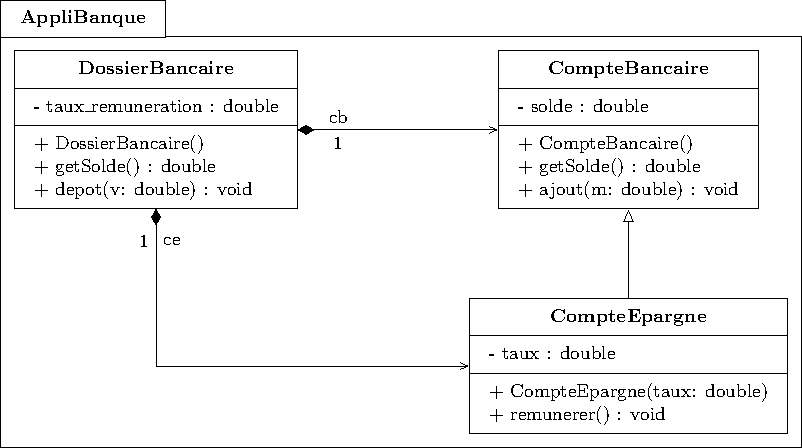
\includegraphics{Diagrammes/UML_UC1.pdf}
    \caption{Diagramme de classes\label{UC1}}
\end{figure}

\newpage 


\subsection{Q2}

La figure~\ref{US1} présente le premier diagramme de séquences imaginé. 
\begin{figure}[h]
    \centering
    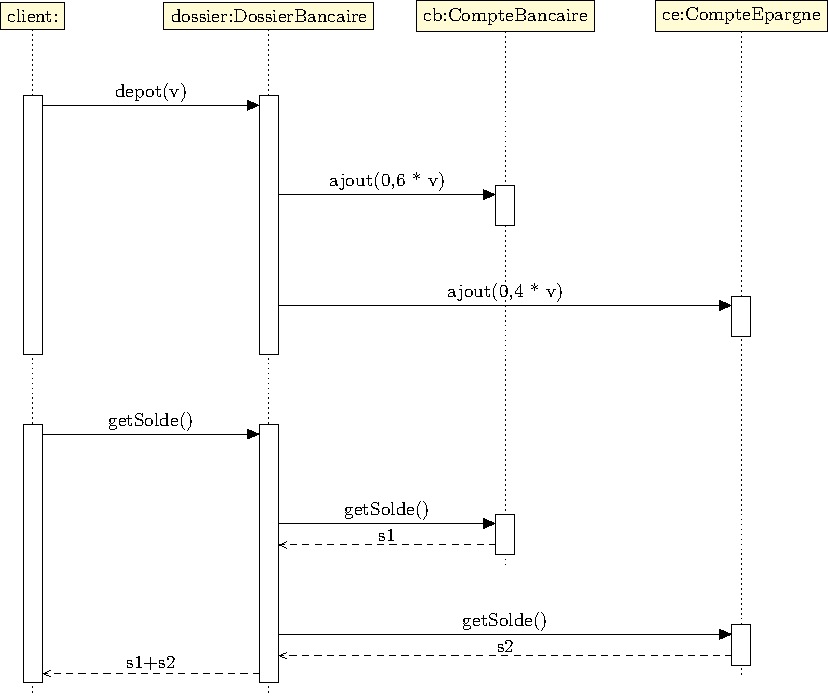
\includegraphics[height=8cm]{Diagrammes/UML_US1.pdf}
    \caption{Diagramme de séquence\label{US1}}
\end{figure}


\subsection{Q3}

En plus des diagrammes précédents, on peut faire un diragramme d'objets modélisant l'état du programme après l'instanciation de l'objet de la classe DossierBancaire.
La figure~\ref{UO1} présente un tel diagramme. 
\begin{figure}[h]
    \centering
    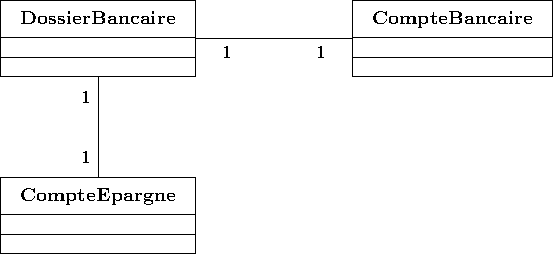
\includegraphics[height=3cm]{Diagrammes/UML_UO1.pdf}
    \caption{Diagramme d\textquotesingle objets\label{UO1}}
\end{figure}

% Exercice 2
\section{Exercice 2}

Pour la compilation du projet simplement, les commandes trouvées 
dans le README permettent de compiler le projet, comme montré dans la figure \ref{ScreenE2Q31}.

\begin{lstlisting}[language=bash]
javac AppliBanque/Main.java
java AppliBanque/Main
\end{lstlisting}

\begin{figure}[h]
    \centering
    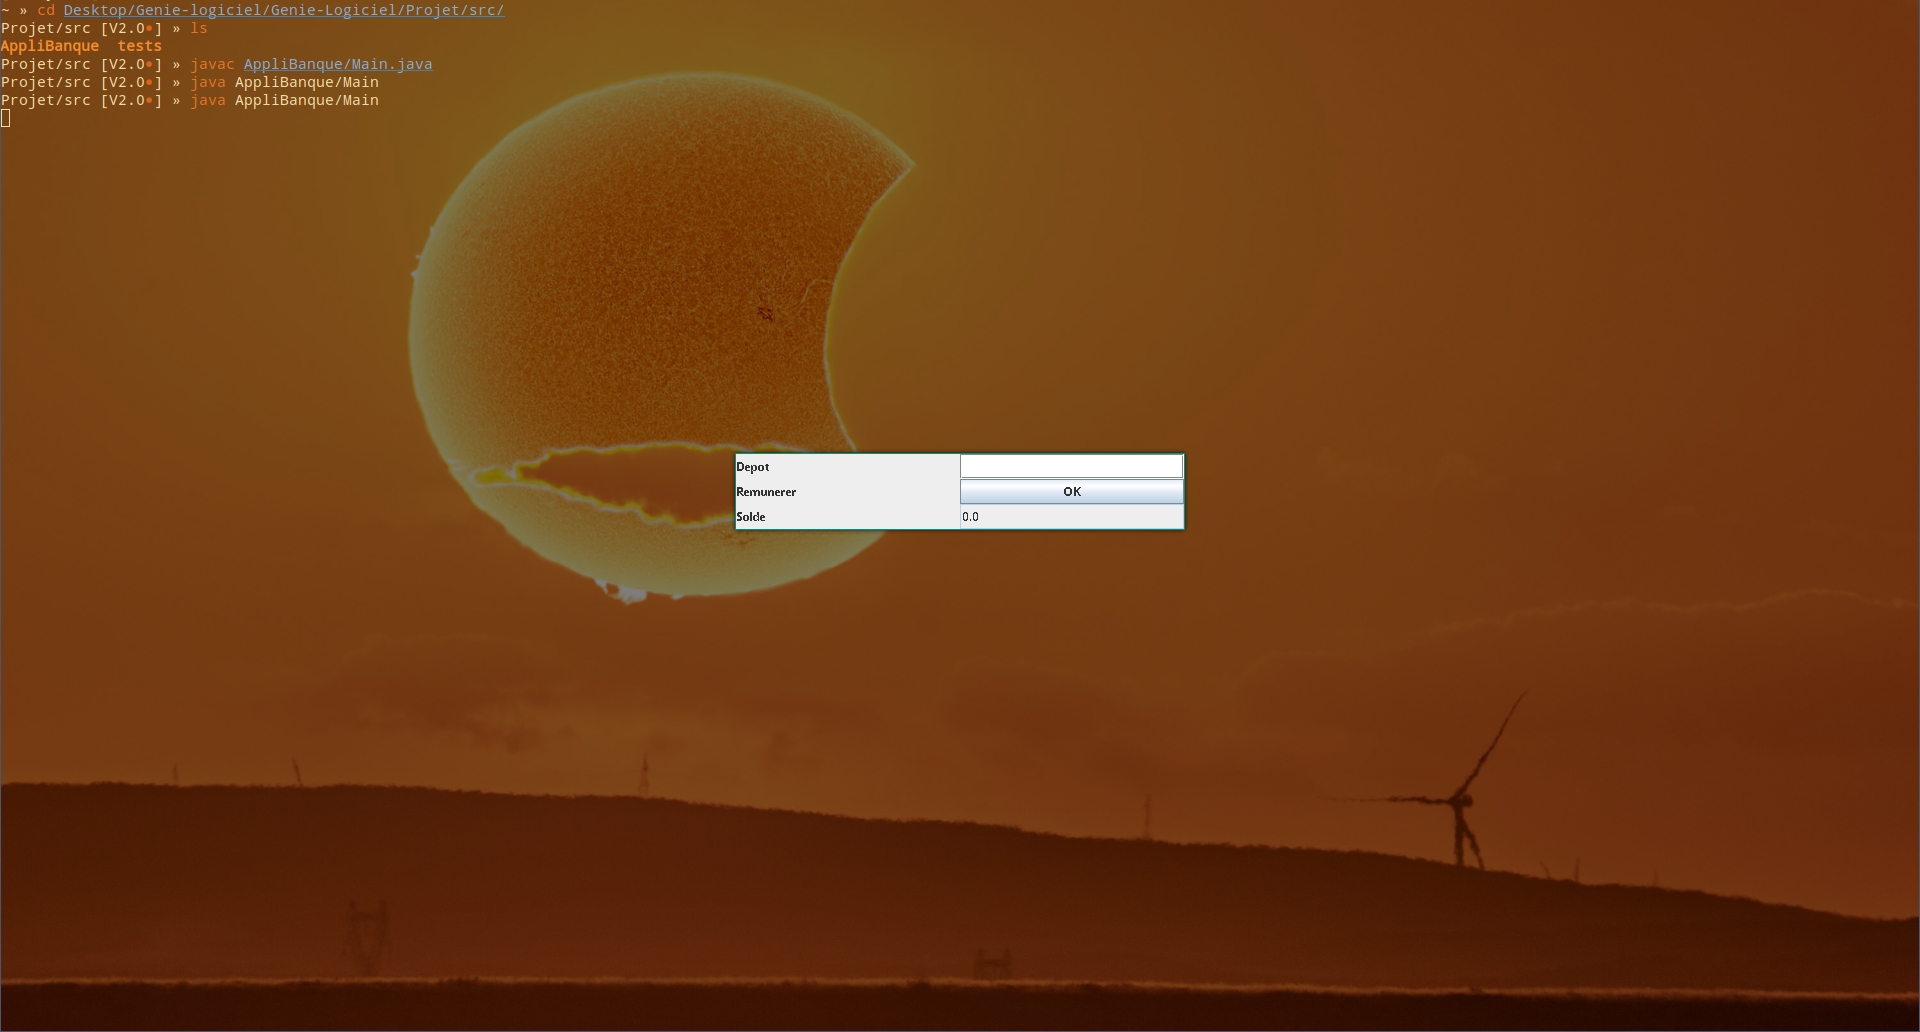
\includegraphics[width=\textwidth]{img/Screenshots/E2_Q3_1.png}
    \caption{Compilation du programme\label{ScreenE2Q31}}
\end{figure}

Pour la compilation des tests, il faut d'abord télécharger JUnit 4 et hamcrest-core et placer les fichiers .jar
à un endroit connu (l'emplacement du projet par exemple). En utilisant les commandes du README en adaptant les 
chemins en fonction de l'emplacement local, on peut compiler et exécuter les tests.

\begin{lstlisting}[language=bash]
    javac --classpath "chemin/vers/juint.jar":"chemin/vers/hamcrest.jar": tests/TestAppliBanque.java
    java --classpath "chemin/vers/juint.jar":"chemin/vers/hamcrest.jar": tests/TestAppliBanque
\end{lstlisting}

% Exercice 3
\section{Exercice 3}

\subsection{Q1-Q2}

Pour travailler parallèlement sur le projet, nous avous utilisé le logiciel de versionning git couplé à un outil 
de dépôt en ligne appelé GitHub. Les étapes effectuées pour initialiser le dépôt sont:
\begin{itemize}
    \item Création de l'arboresence des fichiers, avec un dossier "Projet" contenant le code Java, et un dossier "Rapport" contenant le rapport
    \item Ecriture du fichier .gitignore, permettant de ne pas avoir de fichiers inutiles dans le dépôt, notamment le bytecote généré par Java et les fichiers de log de \LaTeX.
    \item Initialisation du dépôt local avec la commande \textquotesingle git init\textquotesingle
    \item Ajout des fichiers à prendre en compte dans le commit avec \textquotesingle git add .\textquotesingle 
    \item Commit la version de départ avec \textquotesingle git commit -m "Commit initial"\textquotesingle 
    \item Création du dépôt distant sur github avec l'utilitaire invoqué par la commande\textquotesingle gh repo create\textquotesingle 
    \item Push du contenu local sur le dépôt distant avec \textquotesingle git push -u origin master\textquotesingle 
\end{itemize}

Par la suite, nous avons effectué les différents commits via la console en ajoutant des tags quand 
nécéssaire avec la commande \textquotesingle git tag\textquotesingle .
Pour ajouter les tags dans le dépôt distant, il faut exécuter la commande \textquotesingle git push origin --tags\textquotesingle

\subsection{Q3}

\begin{lstlisting}[language=Java]
// TestDossierBancaire.java
@Test
public void test_constructeur() 
{
	DossierBancaire dossier=new DossierBancaire();
	assertNotNull(dossier);
}

@Test  
public void test_deposer() 
{
	DossierBancaire dossier=new DossierBancaire();
	dossier.deposer(100);
	assertEquals(100,dossier.get_solde(),0); 
}

@Test
public void test_remunerer() 
{
	DossierBancaire dossier=new DossierBancaire();
	dossier.deposer(100);
	dossier.remunerer();
	double apres_remuneration = 0.4 * 100 + 0.6 * 100 * 1.032;
	assertEquals(apres_remuneration,dossier.get_solde(),0);
}
\end{lstlisting}

L'exécution de ces tests fonctionne sauf pour rémunérer qui n'a pas encore été implémentée, comme montré sur la figure \ref{ScreenE3Q31}.
\begin{figure}[h]
    \centering
    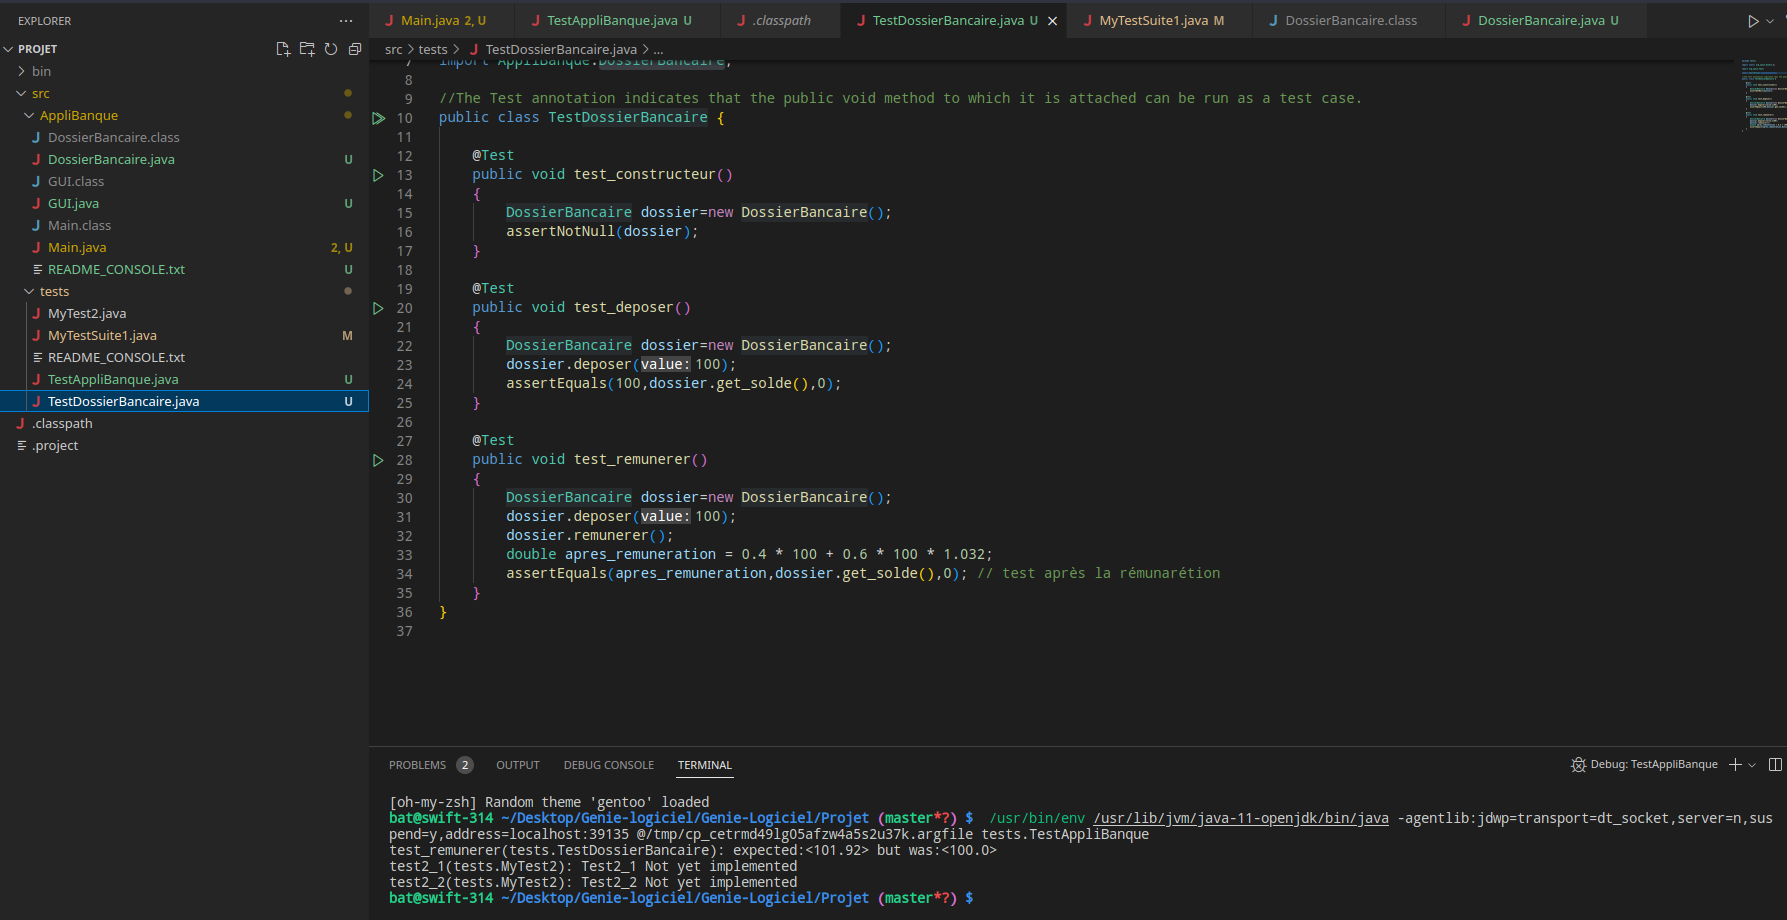
\includegraphics[width=\textwidth]{img/Screenshots/E3_Q3_1.png}
    \caption{Tests\label{ScreenE3Q31}}
\end{figure}

\subsection{Q5}

\begin{lstlisting}
// CompteBancaire.java
...
public class CompteBancaire {

    protected double m_solde;

    public CompteBancaire()
    {
        m_solde=0;
    }
    public void deposer(double value) {m_solde+=value;}
    public double get_solde() {return m_solde;}

}
\end{lstlisting}

\begin{lstlisting}
// DossierBancaire.java
...
public class DossierBancaire {
    
    private CompteBancaire m_compte_bancaire;

    //Constructeur
    public DossierBancaire()
    {
        m_compte_bancaire = new CompteBancaire();
    }

    public void deposer(double value) {m_compte_bancaire.deposer(value);}
    public void getSolde() {return m_compte_bancaire.getSolde();}
    public void remunerer() {}
    
}
\end{lstlisting}

\subsection{Q6}

\begin{lstlisting}
// CompteEpargne.java
...
public class CompteEpargne extends CompteBancaire {

    private double taux;
    public CompteEpargne(double t)
    {
        taux = 1+t/100;
    	m_solde=0;
    }

    public void remunerer(){m_solde = m_solde * taux;}
}
\end{lstlisting}

Lors de l'implémentation de CompteEpargne dans DossierBancaire, nous n'avons pas utilisé de variable taux\_remuneration (comme indiqué dans le diagramme UML). A la place, le taux est écrit en dur dans le constructeur de CompteEpargne.
La version finale du diagramme de classes est disponible à la figure~\ref{UC2}.

\begin{lstlisting}
// DossierBancaire.java
...
public class DossierBancaire {
    
    private CompteEpargne m_compte_epargne;
    private CompteBancaire m_compte_bancaire;

    //Constructeur
    public DossierBancaire()
    {
        m_compte_bancaire = new CompteBancaire();
        m_compte_epargne = new CompteEpargne(3.2);
    }

    public void deposer(double value) {
        m_compte_bancaire.deposer(value*0.4);
        m_compte_epargne.deposer(value*0.6);
    }
    public void getSolde() {return m_compte_bancaire.getSolde() + m_compte_epargne.getSolde();}
    public void remunerer() {m_compte_epargne.remunerer();}
    
}
\end{lstlisting}

Les tests sont déjà adaptés à l'implémentation du compte épargne, et réussisent maintenant car le compte épargne est implémenté.

% Exercice 4
\section{Exercice 4}

\subsection{Q1}
On a rajouté quelques commentaires dans la classe DossierBancaire.

\subsection{Q2}

Le retour à une version précédente se fait via la commande
\begin{lstlisting}[language=bash]
git checkout V2.0
\end{lstlisting}
(pour retourner au commit avec le tag V2.0 par exemple)\\ \\
La création de la nouvelle branche à partir de V2.0 se fait avec la commande
\begin{lstlisting}[language=bash]
git branch new_dev
\end{lstlisting}
Pour se rendre sur la branche (déplacer la HEAD sur la branche), il faut faire la commande
\begin{lstlisting}[language=bash]
git checkout new_dev
\end{lstlisting}

\subsection{Q3}

Pour retourner sur la branche principale (déplacer la HEAD sur la branche), il faut faire la commande
\begin{lstlisting}[language=bash]
git checkout master
\end{lstlisting}

\subsection{Q4}

L'intégration des modification apportees dans new\textunderscore dev sur la branche master se fait au moyen d'un merge.
Ce dernier s'effectue avec la commande:
\begin{lstlisting}[language=bash]
git merge new_dev master
\end{lstlisting}

\subsection{Q5}
Nous n'avons pas eu d'erreur de fusion, et après exécution le programme fonctionne normalement.


% Exercice 5
\section{Exercice 5}

\subsection{Q1}

L'ajout de la possibilité de retirer de l'argent se fait dans le Compte Bancaire.
La vérification du solde se fait de dans Dossier Bancaire.

\begin{lstlisting}
// CompteBancaire.java
...
public void retirer(double value) {m_solde = m_solde - value;}
...
\end{lstlisting}

\begin{lstlisting}
// DossierBancaire.java
...
public void retirer(double value) throws Exception
{
    if(value > m_compte_bancaire.getSolde()) {
        throw new Exception("Pas assez d'argent sur le compte bancaire");
    }else{
        m_compte_bancaire.retirer(value);
    }
}
...
\end{lstlisting}

\subsection{Q2}

Les tests unitaires testent le cas où suffisament d'argent et présent et le cas inverse.

\begin{lstlisting}
// TestSuite.java
...
public class TestSuite {

	@Test  
	public void test_retirer_suffisant() throws Exception 
	{
		DossierBancaire dossier=new DossierBancaire();
		dossier.deposer(100);
		dossier.retirer(20);
		assertEquals(80,dossier.get_solde(),0); 
	}

	@Test
	public void test_retirer_insuffisant() 
	{
		DossierBancaire dossier=new DossierBancaire();
		dossier.deposer(100);
		try {
			dossier.retirer(41);
		} catch (Exception e) {
			//e.printStackTrace();
			fail("Insuffisance dans le compte Bancaire");
		}
		
	}

}
\end{lstlisting}

\subsection{Q3}

Pour le GUI, on a recopié et réutilisé le code existant pour rajouter un bouton et un text field qui permettent d'appeler la fonction retirer.

\section{Conclusion}

Lors du projet, nous avons implémenté et programmé d'une façon qui diffère du modèle proposé dans le diagramme de classe décrit à la figure~\ref{UC1}.
Finalement, notre programme peut être modélisé selon le diagramme de classes de la figure~\ref{UC2}.

\begin{figure}[h]
    \centering
    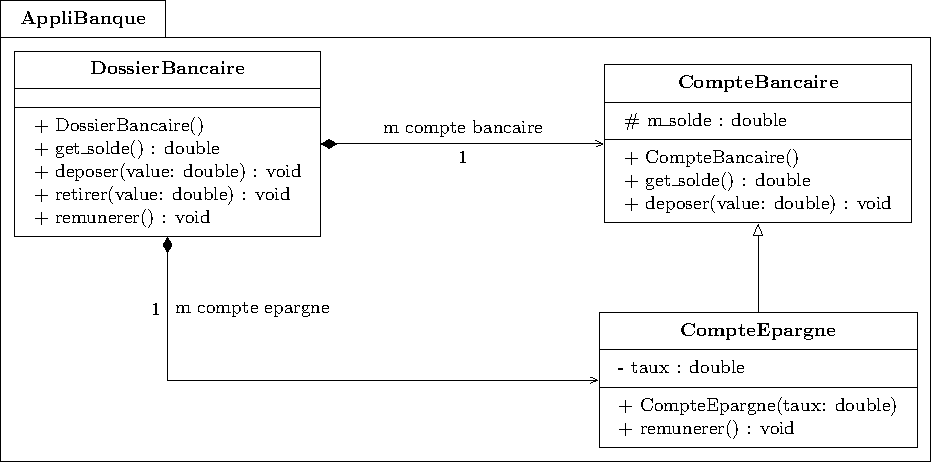
\includegraphics{Diagrammes/UML_UC2.pdf}
    \caption{Diagramme de classes final\label{UC2}}
\end{figure}

Le rapport du TD a été réalisé sur une branche différente du projet qui a été fusionnée à la toute fin.

\end{document}